%-----------------------------------------------------------------------------%
\chapter{ANALISIS DAN PERANCANGAN SISTEM}
%-----------------------------------------------------------------------------%

%
\vspace{4.5pt}

\noindent Bab ini memaparkan analisis masalah yang diatasi berserta pendekatan dan alur kerja dari perangkat lunak yang dikembangkan, mengimplementasikan metode yang digunakan dan hasil yang akan ditampilkan.
\\
\section{Analisis Masalah}
\noindent Pada bab 1 telah dijelaskan bahwa penelitian mengenai sistem pengenalan plat nomor kendaraan merupakan bidang yang masih berkembang dan implementasinya memegang peranan penting dalam bidang transportasi. Pada penelitian ini, metode yang akan digunakan adalah \textit{Hough Transform} untuk mendeteksi lokasi plat kendaraan, kemudian menggunakan metode \textit{Histogram of Oriented Gradient} untuk mengekstraksi fitur dari citra karakter dari plat nomor yang sudah disegmentasi dengan menghitung grafik horizontal pita, kemudian dilakukan klasifikasi dengan menggunakan metode \textit{Support Vector Machine}.
\noindent Masukan untuk sistem deteksi dan pengenalan plat nomor kendaraan ini adalah citra yang ditangkap oleh kamera DSLR Canon EOS 500 D dan Canon EOS 550 D beresolusi 15 dan 18 megapiksel. Citra tangkapan kemudian akan diubah resolusinya menjadi 1024 $\times$ 640 piksel. Setiap citra masukan berisi bagian depan dari kendaraan yang memiliki plat nomor kendaraan.
\noindent Keluaran atau hasil dari sistem akan berupa teks hasil dari pengenalan karakter pada citra plat nomor kendaraan masukan.\\ 

\section{Kerangka Pemikiran}
\noindent Berikut ini adalah kerangka pemikiran dari metode yang diusulkan untuk melakukan deteksi plat nomor kendaraan dan melakukan pengenalan karakter pada citra karakter yang terdapat pada plat nomor.
\\
\begin{adjustbox}{width=1\textwidth}
	\noindent
	\begin{minipage}{\linewidth}
		\framebox[\textwidth]{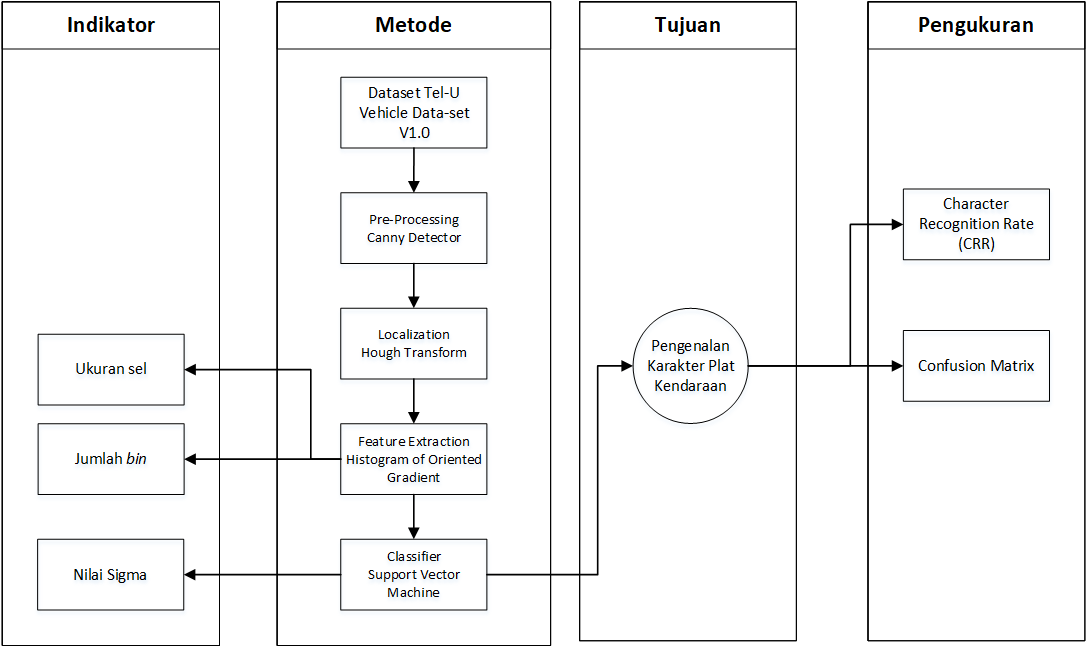
\includegraphics[width=13cm]{images/KerangkaPemikiran.png}}
		\captionof{figure}{Kerangka Pemikiran}
		\label{fig:KerangkaPemikiran}
	\end{minipage}
\end{adjustbox}

\noindent Seperti pada gambar \ref{fig:KerangkaPemikiran}, terdapat beberapa variabel indikator yang memengaruhi hasil dan perlu dilakukan penyesuaian, seperti ukuran sel pada metode \textit{Histogram of Oriented Gradient}, jumlah \textit{bin} yang menentukan batasan sudut yang digunakan, dan nilai sigma untuk \textit{classifier} \textit{Support Vector Machine}. Penelitian ini memiliki tujuan untuk menerapkan \textit{Histogram of Oriented Gradient} dan \textit{Support Vector Machine} untuk sistem pengenalan karakter pada plat nomor dengan menguji beragam faktor yang diduga akan mempengaruhi hasil akurasi dari penggabungan kedua metode tersebut. Hasil pengenalan karakter akan diukur dengan menggunakan \textit{Confusion Matrix}.\\

\section{Urutan Proses Global}
\noindent Dalam sistem pengenalan plat nomor kendaraan terbagi atas dua proses yaitu proses \textit{training} dan proses \textit{testing}. Proses \textit{training} dilakukan untuk mendapatkan kelas-kelas dari karakter-karakter yang akan dikenali. Proses \textit{testing} dilakukan untuk menghitung hasil yang berupa akurasi dari pengenalan karakter pada plat nomor kendaraan.\\

\begin{adjustbox}{width=1\textwidth}
	\noindent
	\begin{minipage}{\linewidth}
		\framebox[\textwidth]{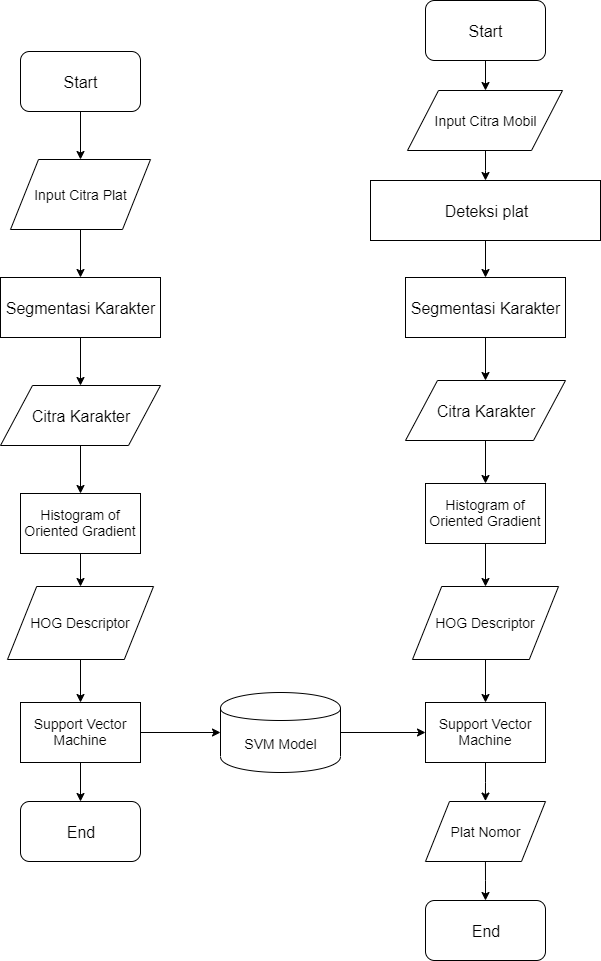
\includegraphics[width=12cm]{images/FlowchartGlobal.png}}
		\captionof{figure}{\textit{Flowchart Global} Sistem Pengenalan Plat Nomor Kendaraan\\}
		\label{fig:FlowchartGlobal}
	\end{minipage}
\end{adjustbox}

\noindent Seperti pada gambar \ref{fig:FlowchartGlobal}. Bagian kiri merupakan \textit{flowchart} dari proses \textit{training} dan bagian kanan merupakan \textit{flowchart} dari proses \textit{testing}. Berikut ini adalah uraian dari proses-proses yang terjadi ketika tahapan \textit{training}:
\begin{enumerate}
	\item Citra masukan adalah citra plat nomor kendaraan mobil yang di-\textit{crop} secara manual dari citra mobil utuh hal ini untuk memastikan citra yang didapatkan adalah plat yang benar. 
	\item Citra plat kemudian akan melalui tahapan \textit{preprocessing} yang meliputi \textit{grayscaling} untuk menghilangkan informasi warna yang tidak diperlukan, \textit{Gaussian Smoothing} untuk menghilangkan derau pada citra, \textit{Binarization} untuk mengubah citra menjadi citra biner, menghilangkan objek kecil (untuk menghilangkan objek seperti baut pada plat) dengan cara menghilangkan objek yang luasnya kurang dari \textit{threshold} sebesar 100 piksel, dan terakhir \textit{Inverse Binarization} untuk mendapatkan citra karakter berwarna hitam dengan latar belakang berwarna putih.
	\item Citra plat selanjutnya melalui tahapan segmentasi karakter, tahapan segmentasi bertujuan untuk mendapatkan citra-citra karakter dari plat nomor tersebut tahapan segmentasi dilakukan dua tahapan, yaitu segmentasi horizontal dan segmentasi vertikal.
	\item Citra karakter hasil \textit{segmentasi} akan di-\textit{scaling} menjadi berukuran 32 $\times$ 32 piksel. Kumpulan karakter yang digunakan adalah karakter angka dari 0 sampai dengan 9 dan karakter huruf dari A sampai dengan Z, tidak ada karakter huruf kecil dikarenakan plat nomor kendaraan tidak ada yang menggunakan karakter huruf kecil.
	\item \textit{Histogram of Oriented Gradient} berfungsi untuk mendapatkan fitur dari citra hasil segmentasi. Hasil dari ekstraksi fitur dengan menggunakan HOG adalah \textit{HOG descriptor}, yang mendeskripsikan distribusi dari gradien berarah pada suatu area citra.
	\item Untuk ukuran sel dan jumlah \textit{bin} yang digunakan untuk proses ekstraksi fitur dengan menggunakan \textit{HOG}, dikarenakan kedua parameter tersebut merupakan indikator uji seperti ditunjukan pada kerangka pemikiran \ref{fig:KerangkaPemikiran}, maka nilai dari ukuran sel dan jumlah \textit{bin} akan menyesuaikan dengan kondisi yang akan diuji.
	\item Setelah tahapan ekstraksi fitur, fitur-fitur akan disimpan dalam berkas CSV dan proses pelabelan fitur untuk setiap karakter akan dilakukan terhadap berkas CSV tersebut.
	\item \textit{Support Vector Machine} (SVM) digunakan untuk mengklasifikasikan fitur-fitur yang sudah didapatkan ke dalam kelas-kelas dari karakter yang akan dikenali. Metode \textit{SVM} yang digunakan pada penelitian ini berasal dari \textit{library WEKA}.
\end{enumerate}
%\subsection{Proses \textit{Training}}
%\begin{adjustbox}{width=1\textwidth}
%	\noindent
%	\begin{minipage}{\linewidth}
%		\framebox[\textwidth]{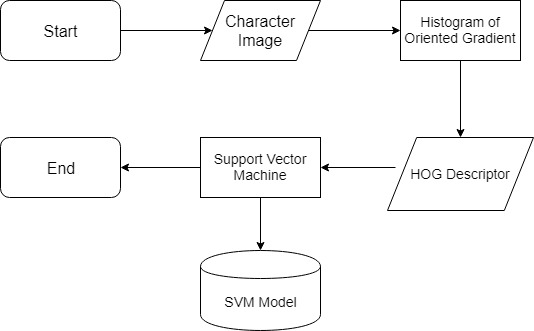
\includegraphics[width=12cm]{images/FlowchartTraining.jpg}}
%		\captionof{figure}{\textit{Flowchart Training} Sistem Pengenalan Plat Nomor Kendaraan\\}
%		\label{fig:FlowchartTraining}
%	\end{minipage}
%\end{adjustbox}
%Berikut ini adalah uraian dari \textit{flowchart} pada gambar \ref{fig:FlowchartTraining} yang dilakukan dalam penelitian ini:
%\begin{enumerate}
%	\item Citra yang menjadi masukkan adalah citra karakter hasil segmentasi dari citra plat nomor kendaraan. Citra karakter masukkan berukuran 32 $\times$ 32 piksel. Citra karakter berwarna hitam dengan latar belakang berwarna putih. Kumpulan karakter yang digunakan adalah karakter angka dari 0 sampai dengan 9 dan karakter huruf dari A sampai dengan Z, tidak ada karakter huruf kecil dikarenakan plat nomor kendaraan tidak ada yang menggunakan karakter huruf kecil.
%	\item \textit{Histogram of Oriented Gradient} berfungsi untuk mendapatkan fitur dari dari citra masukan. Hasil dari ekstraksi fitur dengan menggunakan HOG adalah \textit{HOG descriptor}, yang mendeskripsikan distribusi dari gradien berarah pada suatu area citra.
%	\item Ukuran sel dan blok yang digunakan untuk proses ekstraksi fitur dengan menggunakan \textit{HOG} adalah beragam sesuai dengan ukuran-ukuran sel yang akan digunakan untuk proses testing dan jumlah \textit{bin} yang digunakan juga akan beragam sesuai dengan ukuran \textit{bin} yang digunakan untuk proses testing. Ukuran sudut yang akan dipakai adalah dari 0 sampai dengan 180 derajat.
%	\item \textit{Support Vector Machine} (SVM) digunakan untuk mengklasifikasikan fitur-fitur yang sudah didapatkan ke dalam kelas-kelas dari karakter yang akan dikenali. Metode \textit{SVM} yang digunakan pada penelitian ini berasal dari \textit{library WEKA}.\\
%\end{enumerate}
%
%\subsection{Proses \textit{Testing}}
%\begin{adjustbox}{width=1\textwidth}
%	\noindent
%	\begin{minipage}{\linewidth}
%		\framebox[\textwidth]{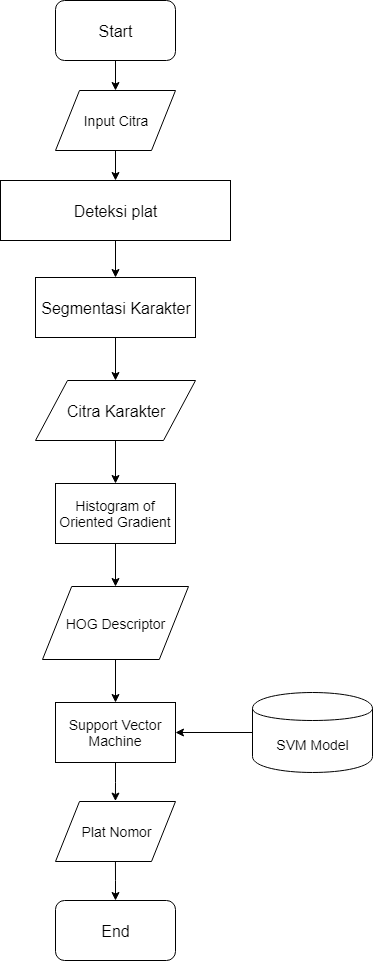
\includegraphics[width=7cm]{images/FlowchartTesting.png}}
%		\captionof{figure}{\textit{Flowchart Testing} Sistem Deteksi dan Pengenalan Plat Nomor\\}
%		\label{fig:FlowchartTesting}
%	\end{minipage}
%\end{adjustbox}
\noindent Kemudian untuk proses \textit{testing}, seperti terlihat pada gambar \ref{fig:FlowchartGlobal}, terdapat beberapa proses yang sama seperti pada proses \textit{training}. Berikut ini adalah uraian dari \textit{flowchart} bagian kanan pada gambar \ref{fig:FlowchartGlobal} yang dilakukan dalam penelitian ini:
\begin{enumerate}
	\item Citra pengujian yang digunakan didapatkan dari \textit{dataset} plat nomor kendaraan Universitas Telkom yang bernama \textit{Tel-U Vehicle Data-set V1.0}, penggunaan dari dataset ini sesuai dengan perizinan dari institusi yang bersangkutan. 
	\item Citra kendaraan akan melalui tahapan deteksi area plat kendaraan untuk mendapatkan citra plat.
	\item Citra plat yang didapatkan kemudian disegmentasi untuk mendapatkan citra karakter. 
	\item Citra yang akan menjadi input dari \textit{HOG} adalah citra hasil dari segmentasi karakter pada citra plat kendaraan hasil deteksi lokasi plat nomor kendaraan.
	\item Ukuran dari sel dan blok yang digunakan untuk proses ekstraksi fitur dengan menggunakan \textit{HOG} akan beragam sesuai dengan pengujian yang akan dilakukan.
	\item Pada tahap \textit{testing} model SVM yang digunakan berasal dari hasil keluaran model SVM pada tahap \textit{training}.
	\item Hasil keluaran akan berupa sebuah \textit{string} yang menunjukkan kumpulan karakter yang berhasil dikenali oleh sistem.\\
\end{enumerate}

\section{Analisis Manual}
\noindent Pada bagian ini dilakukan analisis tahapan proses dengan melakukan perhitungan manual.\\

\subsection{\textit{Dataset}}
\noindent Citra plat kendaraan yang digunakan sebagai dataset adalah citra plat yang di-\textit{crop} secara manual seperti terlihat pada gambar \ref{fig:ContohCitraPlat}.

\begin{adjustbox}{width=1\textwidth}
	\noindent
	\begin{minipage}{\linewidth}
		\framebox[\textwidth]{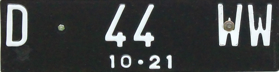
\includegraphics[width=8cm]{images/ContohPlat.PNG}}
		\captionof{figure}{Contoh citra plat yang digunakan\\}
		\label{fig:ContohCitraPlat}
	\end{minipage}
\end{adjustbox}

\noindent Dari citra plat akan dilakukan tahapan \textit{preprocessing}. Hasil akhir dari tahapan-tahapan tersebut dapat dilihat pada gambar \ref{fig:ContohCitraPlatHasilPreprocessing}.

\begin{adjustbox}{width=1\textwidth}
	\noindent\begin{minipage}{\linewidth}
		\framebox[\textwidth]{
\includegraphics[width=8cm]{images/ContohHasilPreprocessing.PNG}}
		\captionof{figure}{Contoh citra plat setelah proses \textit{preprocessing}\\}
		\label{fig:ContohCitraPlatHasilPreprocessing}
	\end{minipage}
\end{adjustbox}

\noindent Dari citra plat hasil \textit{preprocessing}, berikutnya dilakukan proses segmentasi terhadap citra plat. Segmentasi horizontal bertujuan untuk memisahkan area karakter plat nomor dengan karakter tanggal masa berlaku plat nomor. Sedangkan segmentasi vertikal bertujuan untuk mendapatkan karakter karakter. Hasilnya dapat dilihat pada gambar \ref{fig:CitraPlatHasilSegmentasiHorizontal} dan gambar \ref{fig:CitraPlatHasilSegmentasiVertikal}.

\begin{adjustbox}{width=1\textwidth}
	\noindent
	\begin{minipage}{\linewidth}
		\framebox[\textwidth]{
\includegraphics[width=8cm]{images/HasilSegmentasiHorizontal.PNG}}
		\captionof{figure}{Citra plat setelah proses segmentasi horizontal\\}
		\label{fig:CitraPlatHasilSegmentasiHorizontal}
	\end{minipage}
\end{adjustbox}

\begin{adjustbox}{width=1\textwidth}
	\noindent\begin{minipage}{\linewidth}
		\framebox[\textwidth]{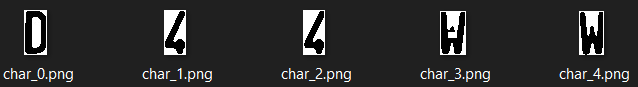
\includegraphics[width=14cm]{images/HasilSegmentasiVertikal.PNG}}
		\captionof{figure}{Citra plat setelah proses segmentasi vertikal\\}
		\label{fig:CitraPlatHasilSegmentasiVertikal}
	\end{minipage}
\end{adjustbox}

\noindent Setelah didapatkan karakter-karakter dari plat nomor tersebut, berikutnya dilakukan proses \textit{scaling} dari ukuran seperti pada gambar \ref{fig:CitraPlatHasilSegmentasiVertikal} menjadi ukuran 32 $\times$ 32 piksel. Alasan digunakannya ukuran 32 $\times$ 32 piksel adalah agar ukuran fitur dari \textit{HOG Descriptor} yang dihasilkan tidak terlalu besar. Hasil dari proses \textit{scaling} citra karakter dapat dilihat pada gambar \ref{fig:ContohCitraDatasetPakai}. Citra karakter hasil proses \textit{scaling} itulah yang akan digunakan sebagai data latih.

\noindent Karakter terdiri dari angka 0 sampai dengan 9 dan karakter huruf kapital dari A sampai dengan Z. Untuk setiap karakter akan digunakan citra latih sebanyak tiga sampai dengan enam citra. Terlihat contoh citra karakter yang ditunjukan pada gambar \ref{fig:ContohCitraDatasetPakai} merupakan contoh karakter angka dan huruf kapital yang akan dipakai.

\begin{adjustbox}{width=1\textwidth}
	\noindent\begin{minipage}{\linewidth}
		\framebox[\textwidth]{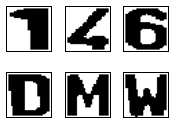
\includegraphics[width=8cm]{images/CitraDatasetPakai.PNG}}
		\captionof{figure}{Contoh citra karakter yang digunakan untuk tahap \textit{training}\\}
		\label{fig:ContohCitraDatasetPakai}
	\end{minipage}
\end{adjustbox}
\\

\subsection{Tahap Pendeteksian Lokasi Plat Nomor}
\noindent Skema alur dari tahap pendeteksian lokasi plat nomor adalah:

\begin{adjustbox}{width=1\textwidth}
	\noindent
	\begin{minipage}{\linewidth}
		\framebox[\textwidth]{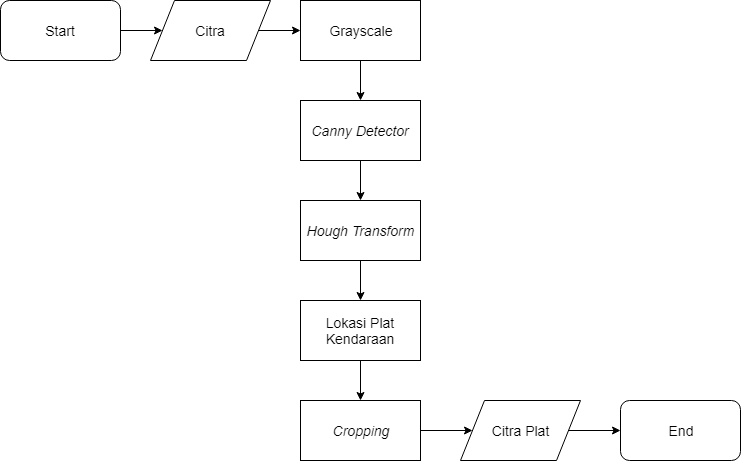
\includegraphics[width=13cm]{images/FlowchartDeteksiPlat.png}}
		\captionof{figure}{Skema Alur Pendeteksian Plat\\}
		\label{fig:SkemaAlurPendeteksianPlat}
	\end{minipage}
\end{adjustbox}\\

\subsubsection{\textit{Grayscale}}
\noindent Proses pertama adalah mengubah citra masukan dari citra RGB menjadi citra \textit{grayscale}, tujuan dari \textit{grayscaling} citra adalah untuk menghilangkan informasi warna dari setiap piksel citra. Untuk menghitung nilai derajat keabuan setiap piksel, diperoleh dengan menggunakan persamaan \ref{eq:grayscale}.
\noindent Di bawah merupakan contoh matriks citra asli dengan 3 \textit{channel} warna yaitu \textit{Red}, \textit{Green}, dan \textit{Blue} berukuran 5 $\times$ 5 piksel. 

\begin{adjustbox}{width=1\textwidth}
	\noindent\begin{minipage}{\linewidth}
		\framebox[\textwidth]{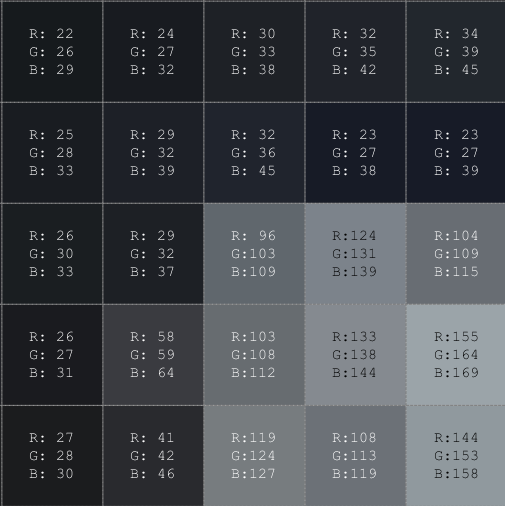
\includegraphics[width=8cm]{images/CitraMatriksAsal.PNG}}
		\captionof{figure}{Matriks Citra Asal berukuran 5 $\times$ 5\\}
		\label{fig:MatriksCitraAsal}
	\end{minipage}
\end{adjustbox} 

\noindent Dengan menggunakan persamaan \ref{eq:grayscale}, maka nilai matriks citra \textit{grayscale} pada titik (4,4) akan menjadi sebagai berikut:
\begin{table}[H]
	\begin{adjustbox}{width=1\textwidth}
		\begin{tabular}{|p{13.55cm}|}
			\hline
			\begin{equation}\nonumber
			\begin{aligned}
			Matriks[4,4] &= (0.299 * 133) + (0.587 * 138) + (0.114 * 144) \\
						 &= 137.189 \approx 137 
			\end{aligned}
			\end{equation}\\
			\hline
		\end{tabular}
	\end{adjustbox}
\end{table}
\noindent Perhitungan di atas dilakukan terhadap seluruh nilai matriks citra asal dan hasilnya adalah matriks citra berukuran 5 $\times$ 5 dengan satu nilai derajat keabuan.

\begin{adjustbox}{width=1\textwidth}
	\noindent\begin{minipage}{\linewidth}
		\framebox[\textwidth]{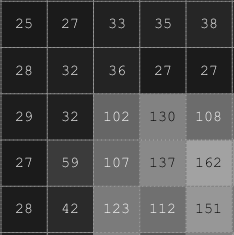
\includegraphics[width=6cm]{images/CitraMatriksGrayscale.PNG}}
		\captionof{figure}{Matriks Citra Hasil \textit{Grayscale}\\}
		\label{fig:MatriksCitraGrayscale}
	\end{minipage}
\end{adjustbox} \\

\subsubsection{Deteksi Tepi Canny}
\noindent Proses deteksi tepi dilakukan terhadap citra hasil \textit{grayscaling}. Pada penelitian ini, metode \textit{Canny Edge Detection} digunakan untuk mendapatkan tepian. Berikut adalah algoritme dari metode \textit{Canny Edge Detection} untuk mendapatkan tepian.
\begin{enumerate}[leftmargin=16pt]
	\item Citra masukan adalah citra dari hasil \textit{grayscaling} pada tahapan sebelumnya.
	\item Citra masukan diperhalus dengan menggunakan \textit{Gaussian Filter} untuk membuang derau.
	\item Lakukan operasi perhitungan gradien menggunakan operator Sobel untuk mendapatkan tepian yang tebal.
	\item Untuk menipiskan tepian yang didapat dari operasi sebelumnya maka teknik \textit{Non-Maxima Suppression} dilakukan dengan mencari nilai maksimum pada tepian.
	\item Buat 2 nilai \textit{threshold} yaitu \textit{high threshold} dan \textit{low threshold} untuk menentukan piksel mana yang masuk dalam kategori tepian kuat, tepian lemah, dan bukan tepian. Jika nilai dari piksel tersebut di atas \textit{high threshold}, maka piksel tersebut masuk ke dalam kategori tepian kuat, apabila nilai piksel berada di antara batas \textit{high threshold} dan \textit{low threshold}, maka piksel tersebut masuk ke dalam kategori tepian lemah, selebihnya akan masuk ke dalam kategori bukan tepian.
	\item Tahapan terakhir adalah \textit{Edge Linking} untuk menghubungkan tepian lemah dengan tepian kuat. Apabila piksel tepian lemah memiliki tetangga piksel (terhubung), maka piksel tersebut akan menjadi tepian.
	\item Citra keluaran adalah citra biner yang merupakan hasil pendeteksian tepi.
	
	\begin{adjustbox}{width=1\textwidth}
		\noindent
		\begin{minipage}{\linewidth}
			\framebox[\textwidth]{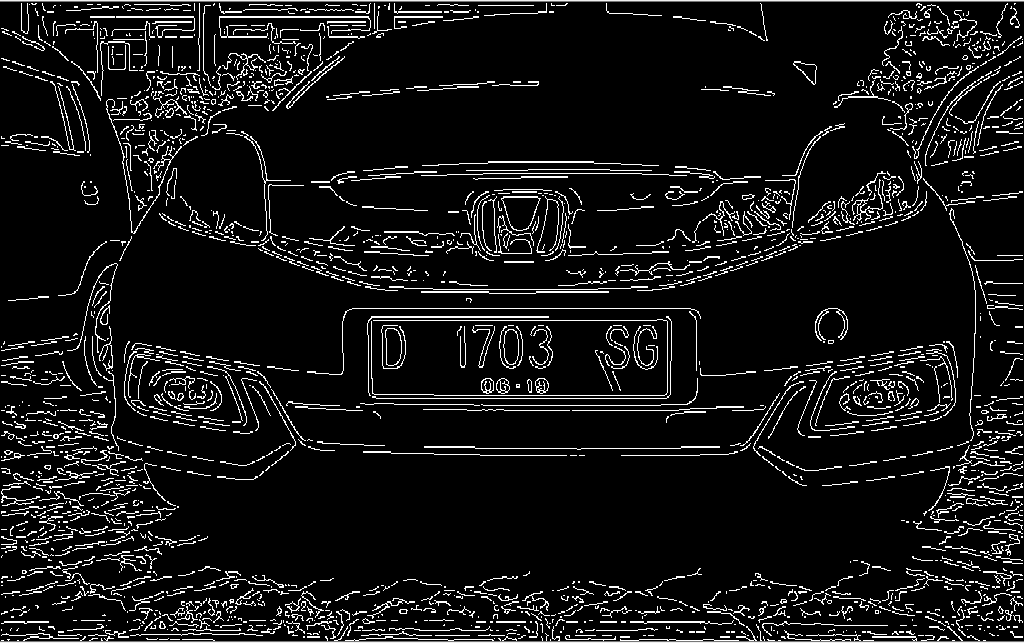
\includegraphics[width=13cm]{images/HasilCanny.png}}
			\captionof{figure}{Contoh Citra hasil deteksi tepi \textit{Canny}\\}
			\label{fig:HasilDeteksiTepi}
		\end{minipage}
	\end{adjustbox}\\
\end{enumerate}

\subsubsection{\textit{Hough Transform}}
\noindent Metode \textit{Hough Transform} yang digunakan adalah untuk identifikasi garis lurus. Dalam ekstraksi fitur \textit{Hough Transform} perlu menspesifikasikan \textit{accumulator space} untuk menyimpan nilai \textit{voting}. Untuk tahapan \textit{Hough Transform} ini akan menggunakan \textit{library} dari \textit{OpenCV} yaitu dengan menggunakan \textit{function} \textit{Imgproc.HoughLines()}. \textit{Function} \textit{Imgproc.HoughLines()} ini memiliki parameter masukan berupa citra biner hasil dari metode \textit{Canny Edge Detection}, \textit{range} sudut yang akan digunakan sebagai $\theta$ untuk membatasi sudut yang akan dicari, dan  nilai rho yang merupakan panjang garis dalam piksel. Spesifikasi \textit{accumulator space} ditentukan berdasarkan ukuran citra input. Berikut adalah algoritme dari metode \textit{Hough Transform} untuk mendapatkan garis lurus:
\begin{enumerate}
	\item Citra masukan adalah citra biner hasil deteksi tepi pada tahapan sebelumnya.
	\item Matriks \textit{Accumulator Space} didefinisikan sebagai \textit{array} 2 dimensi dengan sumbu horizontal menunjukkan nilai sudut ($\theta$) yang digunakan dan sumbu vertikal adalah nilai-nilai dari $\rho$.
	
	\begin{adjustbox}{width=1\textwidth}
		\noindent
		\begin{minipage}{\linewidth}
			\centering\framebox[8cm]{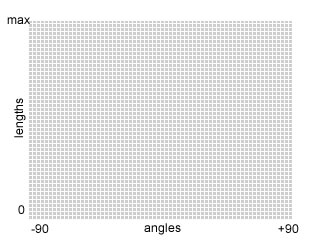
\includegraphics[width=8cm]{images/accumulatorspace.jpg}}
			\captionof{figure}{Ilustrasi matriks \textit{Accumulator Space}\\}
			\label{fig:MatriksAccumulatorSpace}
		\end{minipage}
	\end{adjustbox}
	\item Untuk setiap nilai piksel dari citra biner hasil deteksi tepian, apabila nilai piksel tersebut adalah 0, piksel tersebut diabaikan. Jika nilai piksel tersebut tidak 0, maka lakukan perhitungan nilai $\rho$ untuk piksel tersebut dengan menggunakan persamaan \ref{eq:PersamaanRho} dan lakukan \textit{voting} terhadap setiap nilai $\theta$ yang digunakan dengan menambahkan nilai pada matriks akumulator dengan koordinat ($\theta$, $\rho$) sebesar satu.
	\item Hasil dari perhitungan \textit{voting} akan dicari hasil-hasil \textit{voting} tertinggi untuk dijadikan kandidat garis melalui tahapan pencarian \textit{Hough Peaks}. Tahapan ini dilakukan dengan menentukan nilai \textit{threshold}, \textit{neighbourhood}, dan jumlah \textit{peaks} yang akan diambil.
	\item Hasil pencarian \textit{Hough Peaks} akan menghasilkan kumpulan nilai $\rho$ dan $\theta$, nilai ini kemudian diubah menjadi koordinat titik.
	\item Keluaran dari tahapan ini adalah \textit{array} yang berisi pasangan koordinat titik dari kandidat-kandidat garis yang didapat.\\
\end{enumerate}

\subsubsection{Tahap Validasi Plat Kendaraan}
\noindent Tahap selanjutnya setelah mendapatkan kandidat-kandidat garis adalah menyeleksi area plat nomor. Hal ini dilakukan melalui serangkaian tahapan sebagai berikut:
\begin{enumerate}
	\item Dari keseluruhan kandidat garis yang didapat, pisahkan kandidat garis vertikal dengan kandidat garis horizontal.
	\item Dari kandidat-kandidat garis vertikal akan ada yang menjadi batas kiri dan batas kanan dari area plat kendaraan. Setiap kandidat garis vertikal akan dipasangkan dengan garis vertikal lain dengan cara membandingkan mana garis yang lebih kanan. Hasilnya akan disimpan dalam \textit{array} yang berisi koordinat x dari masing-masing pasangan garis.
	\item Hitung lebar citra yang dibatasi dengan pasangan garis vertikal yang didapatkan, apabila lebar citra sesuai batasan ukuran yang ditentukan, maka pasangan garis tersebut akan menjadi kandidat dari batas kiri dan batas kanan dari plat nomor.
	\item Untuk setiap kandidat batas kiri dan batas kanan plat nomor, pasangkan dengan kandidat garis horizontal dan hitung tinggi citra yang dibatasi dengan batas horizontal, apabila tinggi citra sesuai dengan batasan ukuran yang ditentukan, maka pasangan garis tersebut akan menjadi batas atas dan batas bawah dari citra plat kendaraan.
	\item Jika masih terdapat lebih dari satu kandidat, maka pilih kandidat dengan rasio panjang : lebar yang paling mendekati rasio plat nomor kendaraan Indonesia, yaitu 1 : 3.
	\item Hasil dari tahapan ini adalah 4 titik koordinat yang merupakan koordinat citra plat. Citra plat akan diambil dari citra asal dengan menggunakan titik-titik koordinat tersebut.
\end{enumerate}

\begin{adjustbox}{width=1\textwidth}
	\noindent\begin{minipage}{\linewidth}
		\centering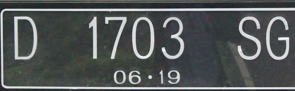
\includegraphics[width=8cm]{images/HasilPlat.png}
		\captionof{figure}{Contoh hasil citra plat\\}
		\label{fig:OutputPlat}
	\end{minipage}
\end{adjustbox}\\

\subsection{Tahapan Segmentasi Karakter}
\noindent Setelah mendapatkan kandidat plat, maka berikutnya dilakukan segmentasi karakter untuk mendapatkan citra-citra karakter yang terdapat pada plat nomor kendaraan. Pada tahapan segmentasi karakter, akan dilakukan dua tahapan, yaitu segmentasi vertikal untuk mendapatkan batas atas dan batas bawah daerah karakter, dan segmentasi horizontal untuk mendapatkan batas kiri dan batas kanan untuk setiap karakter. Untuk tahapan segmentasi karakter ini akan menggunakan \textit{method} dari \textit{library JavaOCR} seperti yang disebutkan pada \ref{tbl:FunctionJavaOCR}, yaitu \textit{LineExtractor.slice()} dan \textit{CharacterExtractor.slice()}. \textit{LineExtractor.slice()} digunakan untuk melakukan segmentasi horizontal, parameter dari \textit{method} tersebut adalah berkas citra plat yang sudah melalui tahapan \textit{preprocessing} dan berkas citra yang akan menampung hasil segmentasi horizontal. Sedangkan \textit{CharacterExtractor.slice()} digunakan untuk melakukan segmentasi vertikal dengan parameter citra hasil segmentasi horizontal, berkas citra yang akan menampung hasil segmentasi vertikal, dan dua parameter berikutnya adalah ukuran lebar dan tinggi citra untuk hasil proses \textit{scaling}. Berikut adalah langkah-langkah dari proses segmentasi karakter:
\begin{enumerate}
\item Citra masukan adalah citra plat hasil tahapan deteksi plat kendaraan yang sudah dilakukan \textit{preprocessing} menjadi citra biner.
\item Lakukan segmentasi vertikal untuk mendapatkan batas atas dan batas bawah dari area kandidat karakter.
\item Lakukan segmentasi horizontal untuk mendapatkan batas kiri dan batas kanan dari setiap citra karakter.
\item Setiap citra karakter yang didapatkan akan di-\textit{scaling} menjadi ukuran 32 $\times$ 32 piksel. Hal ini bertujuan untuk menjaga konsistensi ukuran citra karakter yang digunakan untuk proses \textit{training} dan proses \textit{testing}. Hasil dari segmentasi seperti yang ditunjukkan pada gambar \ref{fig:OutputSegmentasi} ditambahkan satu piksel lebih untuk setiap batas kiri, kanan, atas, dan bawah dari citra, tujuannya adalah agar bentuk karakter yang didapatkan ketika proses ekstraksi fitur dengan menggunakan metode \textit{Histogram of Oriented Gradient} menjadi lebih baik.
\item Keluaran dari tahapan ini adalah citra-citra karakter yang terdapat pada plat nomor.
\end{enumerate}

\noindent Pada penelitian ini, tahapan segmentasi karakter akan menggunakan \textit{library} dari Java OCR dan \textit{method} atau \textit{function} yang digunakan dapat dilihat pada tabel \ref{tbl:FunctionJavaOCR}.\\
\\
\begin{adjustbox}{width=1\textwidth}
	\noindent\begin{minipage}{\linewidth}
		\centering
\includegraphics[width=14cm]{images/OutputSegmentasi.png}
		\captionof{figure}{Contoh hasil keluaran dari tahapan segmentasi\\}
		\label{fig:OutputSegmentasi}
	\end{minipage}
\end{adjustbox}\\

\subsection{\textit{Histogram of Oriented Gradient}}
\noindent Pada proses \textit{Histogram of Oriented Gradients}, masukan untuk proses ini berupa citra yang berasal dari hasil segmentasi. Perhitungan fitur dari metode \textit{Histogram of Oriented Gradient} ini dilakukan per citra karakter hasil segmentasi. Keluaran dari proses ini adalah matriks fitur vektor dari hasil perhitungan \textit{Histogram of Oriented Gradients}. Berikut merupakan langkah-langkah untuk menghitung matriks fitur vektor. Pada gambar dapat dilihat hasil dari proses \textit{resize} dan \textit{crop} citra \textit{grayscale} berukuran 8 $\times$ 4 piksel.

\begin{table}[H]
	\centering
	\begin{small}
		\begin{tabular}{|p{2cm}|p{2cm}|p{2cm}|p{2cm}|}
			\hline
			89 & 92 & 88 & 92 \\
			\hline
			90 & 88 & 90 & 86 \\
			\hline
			91 & 90 & 90 & 94 \\
			\hline
			91 & 122 & 91 & 122 \\
			\hline
			89 & 90 & 89 & 91 \\
			\hline
			90 & 85 & 90 & 86 \\
			\hline
			91 & 90 & 92 & 93 \\
			\hline
			91 & 122 & 91 & 120 \\
			\hline
		\end{tabular}
	\end{small}
	\captionof{figure}{Matriks citra hasil \textit{preprocessing}\\}
	\label{fig:MatriksCitraHasilPreprocessing}
\end{table}

\begin{enumerate}
\item Proses pertama adalah untuk menghitung nilai gradien dari posisi vertikal dan horizontal untuk setiap piksel menggunakan persamaan \ref{eq:PersamaanGradienX} dan \ref{eq:PersamaanGradienY}. Contoh perhitungannya untuk piksel koordinat (2,5) dan hasil dari tahap ini dapat dilihat pada gambar \ref{fig:MatriksCitraHasilGradienX} dan \ref{fig:MatriksCitraHasilGradienY} di bawah:
\begin{equation*}
	G_{x}(2,5) = 89 - 89 = 0
\end{equation*}
\begin{equation*}
	G_{y}(2,5) = 85 - 122 = -37
\end{equation*}
\begin{table}[H]
	\centering
	\begin{small}
		\begin{tabular}{|p{2cm}|p{2cm}|p{2cm}|p{2cm}|}
			\hline
			92 & -1 & 0 & -88 \\
			\hline
			88 & 0 & -2 & -90 \\
			\hline
			90 & -1 & 4 & -90 \\
			\hline
			122 & 0 & 0 & -91 \\
			\hline
			90 & 0 & 1 & -89 \\
			\hline
			85 & 0 & 1 & -90 \\
			\hline
			90 & 1 & 3 & -92 \\
			\hline
			122 & 0 & -2 & -91 \\
			\hline
		\end{tabular}
	\end{small}
	\captionof{figure}{Matriks hasil Perhitungan Gradien sumbu X\\}
	\label{fig:MatriksCitraHasilGradienX}
\end{table}
\begin{table}[H]
	\centering
	\begin{small}
		\begin{tabular}{|p{2cm}|p{2cm}|p{2cm}|p{2cm}|}
			\hline
			90 & 88 & 90 & 86 \\
			\hline
			2 & -2 & 2 & 2 \\
			\hline
			1 & 34 & 1 & 36 \\
			\hline
			-2 & 0 & -1 & -3 \\
			\hline
			-1 & -37 & -1 & -36 \\
			\hline
			2 & 0 & 3 & 2 \\
			\hline
			1 & 37 & 1 & 34 \\
			\hline
			-91 & -90 & -92 & -93 \\
			\hline
		\end{tabular}
	\end{small}
	\captionof{figure}{Matriks hasil Perhitungan Gradien sumbu Y\\}
	\label{fig:MatriksCitraHasilGradienY}
\end{table}
\item Untuk setiap piksel, hitung \textit{magnitude} gradien dan arah gradien menggunakan persamaaan \ref{eq:PersamaanMagnitude} dan \ref{eq:PersamaanArah}. Contoh perhitungannya untuk piksel koordinat (2,5) dan hasil dari tahap ini dapat dilihat pada gambar \ref{fig:MatriksHasilMagnitude}:
\begin{equation*}
M(2,5) = \sqrt{0^2 + (-37)^2} = 37
\end{equation*}
\begin{equation*}
\theta(2,5) = arctan\frac{-37}{0} \approx 90
\end{equation*}
\begin{table}[H]
	\centering
	\begin{small}
		\begin{tabular}{|p{2cm}|p{2cm}|p{2cm}|p{2cm}|}
			\hline
			128.70 & 88.01 & 90 & 123.05 \\
			\hline
			88.03 & 2 & 2.83 & 90.02 \\
			\hline
			90.01 & 34.02 & 4.12 & 96.93 \\
			\hline
			122.02 & 0 & 1 & 91.05 \\
			\hline
			90.01 & 37 & 1.41 & 96.01 \\
			\hline
			85.02 & 0 & 3.16 & 90.02 \\
			\hline
			90.01 & 37.01 & 3.16 & 98.08 \\
			\hline
			152.2 & 90 & 92.02 & 130.12 \\
			\hline
		\end{tabular}
	\end{small}
	\captionof{figure}{Matriks hasil Perhitungan \textit{Magnitude}\\}
	\label{fig:MatriksHasilMagnitude}
\end{table}
\begin{table}[H]
	\centering
	\begin{small}
		\begin{tabular}{|p{2cm}|p{2cm}|p{2cm}|p{2cm}|}
			\hline
			44.37 & 90.65 & 89.99 & 135.66 \\
			\hline
			1.30 & 90.03 & 135 & 178.73 \\
			\hline
			0.64 & 91.69 & 14.04 & 158.19 \\
			\hline
			179.06 & 0 & 90.06 & 1.89 \\
			\hline
			179.36 & 90 & 135 & 22.02 \\
			\hline
			1.35 & 0 & 71.57 & 178.73 \\
			\hline
			0.64 & 88.45 & 18.44 & 159.72 \\
			\hline
			143.28 & 90 & 88.76 & 45.62 \\
			\hline
		\end{tabular}
	\end{small}
	\captionof{figure}{Matriks hasil Perhitungan Arah\\}
	\label{fig:MatriksHasilPerhitunganArah}
\end{table}
\item Kemudian, tentukan ukuran sel, ukuran blok dan jumlah \textit{oriented histogram bins}. Pada penelitian Dalas dan Triggs untuk mendeteksi pejalan kaki sebelumnya, didapat bahwa ukuran sel sebesar 8 $\times$ 8 piksel, ukuran blok sebesar 2 $\times$ 2 ukuran sel dan jumlah bin sebanyak 9 sudah dapat menghasilkan akurasi yang dapat mendeteksi pejalan kaki dengan cukup baik dibandingkan dengan ukuran-ukuran lainnya. Untuk contoh perhitungan analisis kali ini jumlah \textit{oriented histogram bins} yang dipakai sebanyak 4 buah, sehingga didapat nilai sudut setiap \textit{histogram bin} yaitu 180 / 4 = 45. Untuk ukuran sel dipilih sebesar 2 $\times$ 2 piksel dan ukuran blok sebesar 2 $\times$ 2 sel. Untuk setiap blok, terdapat \textit{overlapping} sebesar 50\% dari ukuran blok. Dengan demikian akan didapatkan perhitungan sebagai berikut:
\begin{itemize}
\item Jumlah sel adalah 8, terdiri dari 4 sel vertikal dan 2 sel horizontal.
\item Jumlah blok adalah 3, terdiri dari 3 blok vertikal dan 1 blok horizontal.
\end{itemize}
\item Kemudian untuk setiap sel, tentukan perhitungan \textit{Histogram of Oriented Gradient} dengan melakukan \textit{voting} dari arah gradien dan \textit{magnitude} gradien, dimana arah gradien akan menjadi sudut \textit{bin}, dan \textit{magnitude} gradien akan menjadi bobot nilai. Berikut merupakan contoh proses \textit{voting} untuk piksel dengan koordinat (2,5).
\begin{equation*}
M(2,5) = 37
\end{equation*}
\begin{equation*}
\theta(2,5) = 90
\end{equation*}
Sehingga untuk \textit{bin} dengan sudut 90 akan mendapat nilai bobot sebesar 37 yang didapatkan dari nilai gradien \textit{magnitude}-nya.
Lakukan proses tersebut untuk setiap sel sehingga masing-masing sel akan mempunyai \textit{Histogram of Oriented Gradient}. Berikut contoh hasil perhitungan metode \textit{Histogram of Oriented Gradient} pada sel yang terdapat koordinat piksel (2,5) dapat dilihat pada gambar \ref{fig:HasilHOG}.\\
\begin{adjustbox}{width=1\textwidth}
	\noindent\begin{minipage}{\linewidth}
		\framebox[\textwidth]{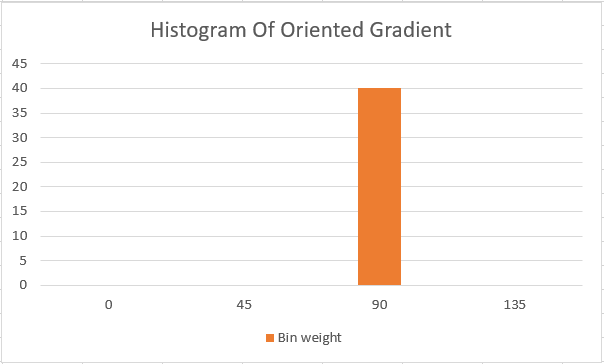
\includegraphics[width=12cm]{images/HistogramOfOrientedGradient.PNG}}
		\captionof{figure}{Contoh hasil \textit{Histogram of Oriented Gradient} untuk sel yang memiliki piksel dengan koordinat (2,5)}
		\label{fig:HasilHOG}
	\end{minipage}
\end{adjustbox}
\item Kemudian untuk setiap blok, akan dilakukan normalisasi dengan menggabungkan hasil histogram dari setiap sel dalam bloknya. Adapun proses normalisasi dapat menggunakan 4 algoritme yaitu, \textit{L1-Norm}, \textit{L1-Sqrt}, \textit{L2-Norm}, dan \textit{L2-Hys}. Pada penelitian ini, penulis menggunakan algoritme normalisasi \textit{L2-Norm} karena berdasarkan penelitian sebelumnya, hasil yang didapat lebih baik dari algoritme lainnya. Persamaan algoritme untuk proses normalisasi menggunakan \textit{L2-Norm} didapat dengan menggunakan persamaan \ref{eq:L2-Norm}. Di bawah adalah contoh perhitungan normalisasi untuk blok pertama:
\begin{table}[H]
	\centering
	\begin{small}
		\begin{tabular}{|p{1cm}|p{1cm}|p{1cm}|p{1cm}|p{1cm}|p{1cm}|p{1cm}|p{1cm}|}
			\hline
			87.28 & 129.45 & 88.73 & 1.28 & 89.28 & 0 & 89.99 & 126.62 \\
			\hline
			208.2 & 1.27 & 32.74 & 3.82 & 140.04 & 5.11 & 0.99 & 46.96 \\
			\hline
			171.21 & 2.55 & 36.99 & 1.28 & 136.49 & 48.28 & 1.87 & 3.96 \\
			\hline
			116.74 & 2.55 & 125.74 & 124.19 & 55.74 & 132.16 & 91.28 & 44.21 \\
			\hline
		\end{tabular}
	\end{small}
	\captionof{figure}{Matriks hasil Perhitungan Histogram untuk seluruh sel\\}
	\label{fig:MatriksHasilPerhitunganHistogram}
\end{table}
Berdasarkan matriks pada gambar \ref{fig:MatriksHasilPerhitunganHistogram}. Elemen matriks yang akan kita gunakan dalam perhitungan normalisasi ini adalah seluruh elemen baris pertama dan baris kedua.
\begin{equation*}
L2_{Norm} = \sqrt{87.28^2 + 129.45^2 + \ldots + 0.99^2 + 46.96^2} = 361.428
\end{equation*}
Kemudian untuk setiap nilai dari histogram dari sel dalam blok tersebut akan dibagi dengan nilai hasil normalisasinya. Di bawah adalah contoh hasil normalisasi histogram dari sel pertama (matriks hasil perhitungan histogram baris pertama kolom 1-4):
\begin{gather*}
\begin{bmatrix}
0.24148 & 0.35815 & 0.2455 & 0.00353 \\
\end{bmatrix}
\end{gather*}
Lakukan proses normalisasi untuk setiap blok dengan menggeser secara horizontal sejauh 1 kali ukuran sel dan secara vertikal sejauh 1 kali ukuran sel sampai blok tersebut sudah berada di bawah kanan dari citra. Kemudian hasil dari proses normalisasi akan disusun menjadi matriks besar dengan jumlah kolom sebesar  \textit{jumlah bin} $\times$ \textit{lebar blok dalam satuan sel} $\times$ \textit{jumlah pergeseran horizontal} dan jumlah baris sebesar \textit{jumlah pergeseran vertikal} $\times$ \textit{tinggi blok dalam satuan sel} , dengan perhitungan tersebut, dalam analisa saat ini didapatkan ukuran matriks sebesar 6 $\times$ 8. Dalam analisa ini, hasil keluaran dari metode \textit{Histogram of Oriented Gradient} ada sebanyak 48 fitur. Di bawah adalah hasil fitur vektor untuk metode \textit{Histogram of Oriented Gradient} setelah melewati proses normalisasi.\\
\begin{table}[H]
	\centering
	\begin{small}
		\begin{tabular}{|p{1cm}|p{1cm}|p{1cm}|p{1cm}|p{1cm}|p{1cm}|p{1cm}|p{1cm}|}
			\hline
			0.24 & 0.36 & 0.25 & 0.00 & 0.25 & 0.00 & 0.25 & 0.35 \\ \hline
			0.58 & 0.00 & 0.09 & 0.01 & 0.39 & 0.01 & 0.00 & 0.13 \\ \hline
			0.61 & 0.00 & 0.10 & 0.01 & 0.41 & 0.01 & 0.00 & 0.14 \\ \hline
			0.50 & 0.01 & 0.11 & 0.00 & 0.40 & 0.14 & 0.01 & 0.01 \\ \hline
			0.48 & 0.01 & 0.10 & 0.00 & 0.38 & 0.14 & 0.01 & 0.01 \\ \hline
			0.33 & 0.01 & 0.35 & 0.35 & 0.16 & 0.37 & 0.26 & 0.12 \\ \hline
		\end{tabular}
	\end{small}
	\captionof{figure}{Matriks hasil Normalisasi\\}
	\label{fig:MatriksHasilNormalisasi}
\end{table}
Setelah mendapatkan matriks \textit{HOG descriptor} di atas. Langkah berikutnya adalah menjadikan matriks tersebut sebagai vektor. Hal ini dilakukan dengan mengambil setiap baris dari matriks dan memasukkannya ke dalam matriks vektor berukuran 1 $\times$ jumlah fitur. Vektor inilah yang akan dijadikan sebagai masukan bagi metode \textit{Machine Learning} yang akan digunakan dalam penelitian ini.\\
\end{enumerate}

\subsection{\textit{Support Vector Machine}}
\noindent Tahapan terakhir dari sistem deteksi dan pengenalan plat nomor kendaraan adalah klasifikasi karakter. Masukan untuk proses ini berupa fitur \textit{HOG Descriptor} untuk setiap citra karakter plat nomor. Tahapan ini bertujuan untuk mengklasifikasikan fitur-fitur dari \textit{HOG descriptor} yang dihasilkan dari perhitungan metode \textit{Histogram of Oriented Gradient} agar dapat dikenali sebagai karakter. \textit{Support Vector Machine} yang akan digunakan dalam penelitian menggunakan \textit{library} dari Weka SVM. Untuk \textit{function} atau \textit{method} yang digunakan pada \textit{library} tersebut dapat dilihat pada tabel \ref{tbl:FunctionWeka}. \textit{Support Vector Machine} termasuk dalam algoritme \textit{supervised learning}. Konsep dasar dari metode ini adalah untuk menemukan sebuah \textit{separating hyperplane} (bidang) yang dapat memisahkan dua kelas sebagai keputusan klasifikasi. Dalam penelitian ini karakter yang akan dikenali adalah huruf A sampai dengan Z dan angka dari 0 sampai dengan 9 sehingga akan terdapat 36 kelas untuk proses klasifikasi.
%\noindent Tabel \ref{tbl:filteredDataset} merupakan rincian jumlah citra pada masing-masing \textit{dataset} setelah dilakukan pemilihan.
%\begin{table}[H]
%	\centering
%	\begin{small}
%		\captionof{table}{Rincian \textit{Dataset} yang telah dipilih\label{tbl:filteredDataset}}
%		\begin{tabular}{|p{4cm}|p{1cm}|p{3cm}|p{3cm}|}
%			\hline
%			\textbf{Nama \textit{Dataset}} &\textbf{Folder} & \textbf{Jumlah Citra} & \textbf{Jumlah Posisi Manusia}\\
%			\hline
%			\textit{Clothing Store} 			& - & 770 & 1631 \\
%			\hline
%			\multirow{3}{*}\textit{Outdoor}	& 31 & 46 & 218 \\\cline{2-4}
%			& 54 & 84 & 371 \\\cline{2-4}
%			& 56 & 113 & 496 \\\hline
%		\end{tabular}
%	\end{small}
%\end{table}



\newpage